\documentclass[aspectratio=169]{beamer}

% Dependency setup
\usepackage{tikz}
%

% Beamer styling setup
\usetheme{AnnArbor}
\usecolortheme{beaver}
\setbeamercolor{titlelike}{parent=structure,bg=lightgray}
%

% Spacing setup
\setlength{\parindent}{0pt} % No paragraph indenting
\setlength{\parskip}{5pt} % Set spacing between paragraphs
\frenchspacing
\newcommand{\mkspace}{\vspace{19pt}}
\newcommand{\rmspace}{\vspace{-19pt}}
%

\begin{document}
\title{Paraméteres bonyolultság}
\author{Kovács Milán, Nemkin Viktória}
\date{2021. március 16.}

\frame{\titlepage}

\frame{\frametitle{Menetrend}\tableofcontents}


\section{Motiváció}

\begin{frame}
\frametitle{P nyelvosztály definíciója}

A P azoknak a nyelveknek az osztálya, amelyekhez van polinom időkorlátos
algoritmus (determinisztikus Turing-gép), azaz ha létezik olyan p(n) polinom, hogy
az algoritmus \textbf{az n méretű bemeneteken legfeljebb p(n)} lépést tesz.

Szeretnénk minden problémára polinom időkorlátos algoritmusokat adni...

Kérdés: Miért csak a bemenet hosszára figyelünk?

\end{frame}


\begin{frame}
\begin{footnotesize}
\frametitle{Példa: Sűrű / ritka gráfok}

\begin{columns}
\begin{column}{0.5\textwidth}
Sűrű gráf (TODO: Egy kevésbé csúnya gráf.)
\begin{center}
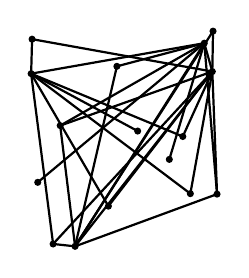
\begin{tikzpicture}[scale=3]
\coordinate (A) at (.772,0.935);
\coordinate (B) at (.225,0.075);
\coordinate (C) at (.806,0.815);
\coordinate (D) at (.039,0.806);
\coordinate (E) at (.162,0.586);
\coordinate (F) at (.624,0.443);
\coordinate (G) at (.826,0.296);
\coordinate (H) at (.402,0.837);
\coordinate (I) at (.067,0.346);
\coordinate (J) at (.809,0.986);
\coordinate (K) at (.132,0.085);
\coordinate (L) at (.366,0.245);
\coordinate (M) at (.681,0.540);
\coordinate (N) at (.713,0.298);
\coordinate (O) at (.490,0.563);
\coordinate (P) at (.043,0.952);

\draw[thick, fill=black] (A) circle (0.01); %node {A};
\draw[thick, fill=black] (B) circle (0.01); %node {B};
\draw[thick, fill=black] (C) circle (0.01); %node {C};
\draw[thick, fill=black] (D) circle (0.01); %node {D};
\draw[thick, fill=black] (E) circle (0.01); %node {E};
\draw[thick, fill=black] (F) circle (0.01); %node {F};
\draw[thick, fill=black] (G) circle (0.01); %node {G};
\draw[thick, fill=black] (H) circle (0.01); %node {H};
\draw[thick, fill=black] (I) circle (0.01); %node {I};
\draw[thick, fill=black] (J) circle (0.01); %node {J};
\draw[thick, fill=black] (K) circle (0.01); %node {K};
\draw[thick, fill=black] (L) circle (0.01); %node {L};
\draw[thick, fill=black] (M) circle (0.01); %node {M};
\draw[thick, fill=black] (N) circle (0.01); %node {N};
\draw[thick, fill=black] (O) circle (0.01); %node {O};
\draw[thick, fill=black] (P) circle (0.01); %node {P};

\draw[thick] (A) -- (B);
\draw[thick] (A) -- (C);
\draw[thick] (A) -- (D);
\draw[thick] (A) -- (E);
\draw[thick] (A) -- (F);
\draw[thick] (A) -- (G);
\draw[thick] (A) -- (H);
\draw[thick] (A) -- (I);
\draw[thick] (B) -- (C);
\draw[thick] (B) -- (E);
\draw[thick] (B) -- (G);
\draw[thick] (B) -- (H);
\draw[thick] (B) -- (J);
\draw[thick] (B) -- (K);
\draw[thick] (C) -- (E);
\draw[thick] (C) -- (G);
\draw[thick] (C) -- (J);
\draw[thick] (C) -- (K);
\draw[thick] (C) -- (L);
\draw[thick] (C) -- (M);
\draw[thick] (C) -- (N);
\draw[thick] (C) -- (P);
\draw[thick] (D) -- (K);
\draw[thick] (D) -- (L);
\draw[thick] (D) -- (M);
\draw[thick] (D) -- (N);
\draw[thick] (D) -- (O);
\draw[thick] (D) -- (P);
\end{tikzpicture}
\end{center}
\end{column}

\begin{column}{0.5\textwidth}
Ritka gráf (TODO: Egy kevésbé csúnya gráf.)
\begin{center}
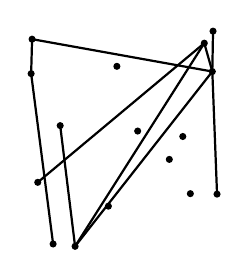
\begin{tikzpicture}[scale=3]
\coordinate (A) at (.772,0.935);
\coordinate (B) at (.225,0.075);
\coordinate (C) at (.806,0.815);
\coordinate (D) at (.039,0.806);
\coordinate (E) at (.162,0.586);
\coordinate (F) at (.624,0.443);
\coordinate (G) at (.826,0.296);
\coordinate (H) at (.402,0.837);
\coordinate (I) at (.067,0.346);
\coordinate (J) at (.809,0.986);
\coordinate (K) at (.132,0.085);
\coordinate (L) at (.366,0.245);
\coordinate (M) at (.681,0.540);
\coordinate (N) at (.713,0.298);
\coordinate (O) at (.490,0.563);
\coordinate (P) at (.043,0.952);

\draw[thick, fill=black] (A) circle (0.01); %node {A};
\draw[thick, fill=black] (B) circle (0.01); %node {B};
\draw[thick, fill=black] (C) circle (0.01); %node {C};
\draw[thick, fill=black] (D) circle (0.01); %node {D};
\draw[thick, fill=black] (E) circle (0.01); %node {E};
\draw[thick, fill=black] (F) circle (0.01); %node {F};
\draw[thick, fill=black] (G) circle (0.01); %node {G};
\draw[thick, fill=black] (H) circle (0.01); %node {H};
\draw[thick, fill=black] (I) circle (0.01); %node {I};
\draw[thick, fill=black] (J) circle (0.01); %node {J};
\draw[thick, fill=black] (K) circle (0.01); %node {K};
\draw[thick, fill=black] (L) circle (0.01); %node {L};
\draw[thick, fill=black] (M) circle (0.01); %node {M};
\draw[thick, fill=black] (N) circle (0.01); %node {N};
\draw[thick, fill=black] (O) circle (0.01); %node {O};
\draw[thick, fill=black] (P) circle (0.01); %node {P};

\draw[thick] (A) -- (B);
\draw[thick] (A) -- (C);
\draw[thick] (A) -- (I);
\draw[thick] (B) -- (C);
\draw[thick] (B) -- (E);
\draw[thick] (C) -- (G);
\draw[thick] (C) -- (J);
\draw[thick] (C) -- (P);
\draw[thick] (D) -- (K);
\draw[thick] (D) -- (P);
\end{tikzpicture}
\end{center}
\end{column}
\end{columns}

Erre a két gráfra nézzünk gráfalgoritmusokat:
\begin{itemize}
\item Legnagyobb független csúcshalmaz.
\item Csúcsszínezés.
\item Stb...
\end{itemize}

Mindkét gráfban ugyanannyi csúcs van, ezért ha szomszédossági mátrixukkal adjuk meg őket, akkor
ugyanakkora lesz az input mérete, azonban a 2. gráfban a fenti kérdésekre elég hamar választ
tudunk adni.
\end{footnotesize}
\end{frame}

\begin{frame}[t]
\frametitle{Példa: Prímtényezős felbontás}

Feladat: számok prímtényezős felbontását megadni.

\mkspace
\begin{columns}
\begin{column}{0.487\textwidth}
$4503599627370496 = 2^{52}$
\end{column}
\begin{column}{0.487\textwidth}
$1125897758834689 = 524287 \cdot 2147483647$
\end{column}
\end{columns}
\mkspace

Ugyanolyan sok számjegyből állnak a számok, tehát ugyanolyan hosszú az input méretünk, mégis az elsőt
nagyon gyorsan meg lehet találni, a másodikat sokkal lassabban.

\end{frame}


\section{Bar Fight Prevention problem}

\begin{frame}
\frametitle{Feladat}
Képzeljük el, hogy biztonsági őrként dolgozunk egy falusi bárban. Péntekenként nagy tömeg szokott lenni és
általában bunyóban végződik a történet... A mi feladatunk kidobni az ittas vendégeket, ami nagyon fárasztó
és nem túl mókás. Elhatározzuk, hogy megelőző intézkedéseket teszünk...

Mindenkit ismerünk a faluban és azt is tudjuk ki kivel nincs jóban, kik fognak várhatóan összeverekedni.
A tervünk tehát az, hogy csak olyan embereket engedünk be a bárba, akik jóban vannak egymással, így
elkerüljük a verekedést.

Azonban a bár menedzsmentje maximalizálni akarja a profitot, ezért azt a kikötést teszi, hogy legfeljebb
$k$ darab vendéget lehet elutasítani az ajtóban.

A feladat tehát a következő: Ismerjük a bárba bejövő emberek listáját ($n$ ember), minden emberpárra
tudjuk, hogy fognak-e verekedni ha mindkettőjüket beengedjük. Ki kell találni, hogy be lehet-e úgy
engedni az embereket, hogy legfeljebb k darab embert utasítunk el, úgy hogy bent ne törjön ki verekedés.
\end{frame}


\begin{frame}

\begin{center}
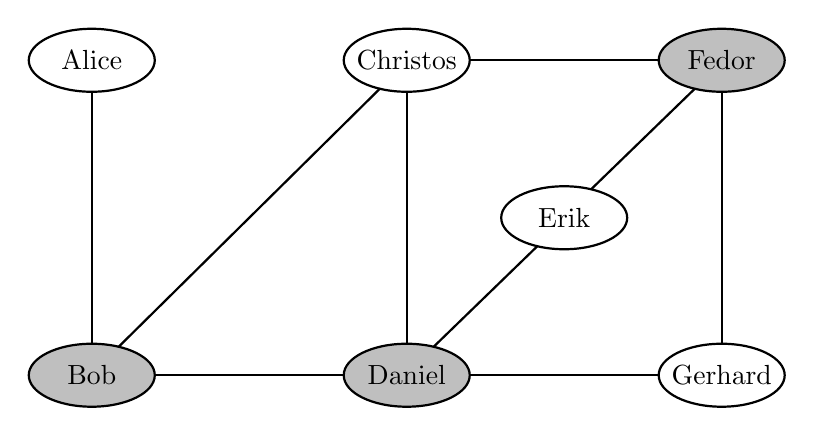
\begin{tikzpicture}[scale=2]
\draw[thick, fill=lightgray] (1,1) ellipse (0.4 and 0.2) node {Bob};
\draw[thick, fill=lightgray] (3,1) ellipse (0.4 and 0.2) node {Daniel};
\draw[thick] (5,1) ellipse (0.4 and 0.2) node {Gerhard};
\draw[thick] (4,2) ellipse (0.4 and 0.2) node {Erik};
\draw[thick] (1,3) ellipse (0.4 and 0.2) node {Alice};
\draw[thick] (3,3) ellipse (0.4 and 0.2) node {Christos};
\draw[thick, fill=lightgray] (5,3) ellipse (0.4 and 0.2) node {Fedor};

\draw[thick] (1.4,1) -- (2.6,1);
\draw[thick] (3.4,1) -- (4.6,1);
\draw[thick] (3.4,3) -- (4.6,3);

\draw[thick] (1,1.2) -- (1,2.8);
\draw[thick] (3,1.2) -- (3,2.8);
\draw[thick] (5,1.2) -- (5,2.8);

\draw[thick] (1.17,1.18) -- (2.83,2.82);
\draw[thick] (3.17,1.18) -- (3.83,1.82);
\draw[thick] (4.17,2.18) -- (4.83,2.82);

\end{tikzpicture}
\end{center}

\end{frame}

\end{document}
